\chapter{Evaluation}
In this chapter, we aim to evaluate the expressiveness of Verlixir's design. First, we perform a qualitative analysis of modelling classical distributed algorithms such as basic Paxos in section \ref{sec:ds}. Then section \ref{sec:vs} will delve into a comparison against current state-of-the-art model checking techniques for modern-day programming languages and verification-aware languages.
\section{Analysing Distributed Systems} \label{sec:ds}
Verifying the correctness of real-world distributed systems is a major motivation for this project. Critical real-time systems (such as in air-traffic control or healthcare  \cite{airlines,healthcare}) should not fail and should rely on rigorous verification techniques to guarantee production code is correct.  
\subsection{Basic Paxos} \label{sec:Paxos}
Paxos is an example of a distributed algorithm \cite{paxos_simple}. It is a consensus algorithm, where many processes are tasked to agree on a value. Processes may propose what this value should be, but only one value should be agreed upon. The safety requirements (SR)s for consensus are:
\begin{itemize}
    \item \textbf{SR1}: Only a value that has been proposed may be chosen.
    \item \textbf{SR2}: Only a single value is chosen.
    \item \textbf{SR3}: A process never learns that a value has been chosen unless it actually has.
\end{itemize}
The system's liveness requirement is that a proposed value is eventually chosen and if a value is chosen then a process can learn the chosen value.
\subsubsection{Informal Specification}
There are many flavours to the Paxos algorithm. We will informally present a basic, one-shot Paxos. We introduce three roles in the system: proposer, acceptor and learner. The Paxos algorithm performs two steps: prepare and accept. A proposer will broadcast a prepare message to all the acceptors, who will respond with a promise. When the proposer has received a promise from a quorum $q$ of acceptors, it will broadcast an accept message. If more than q acceptors accept, then the value is chosen, and the learners are informed.
\par
To evaluate the expressiveness of Verlixir, we first must write the Paxos specification in LTLixir. The specifications of proposer, acceptor and learner are similar to those presented in pseudocode by Marzullo, Mei and Meling \cite{Paxos_pseudocode}. We now present the key differences in our Elixir specification to a traditional Paxos design.
%  For the remainder of the specification, we use the notations $A, \alpha, P, \pi, L, \lambda$ to respectively represent either a set or individual acceptor, proposer or learner.
\par
All processes contain two functions, a start function to introduce relevant initial configuration and a main loop to process messages. Every acceptor initializes an accepted proposal, value and minimum proposal to $-1$ and then processes $prepare$ and $accept$ messages until receiving a $terminate$ message, signifying consensus has been reached. A termination clause is important to ensure the completion of a round of Paxos. A proposer receives its configuration in the form of a $bind$ message, before executing its protocol. If during phase two, when asking acceptors to accept a value, a quorum of acceptors rejects the proposal, the proposer will inform the system it has reached consensus on value $0$. Traditionally, the proposer would retry with a higher proposal number, but we aim to avoid infinite paths so instead introduce this terminating condition. The learner awaits a $learn$ message from all proposers. We only ever consider a single learner and the learner is also responsible for spawning the proposers and acceptors, choosing their values and assigning proposal numbers for the single round of Paxos. We finally setup the learner such that it spawns three acceptors and two proposers. The learner decides the values the proposers will propose, which for this example will be $31$ and $42$. Of course, in a different context, these values may come from other sources within a larger system, however, notional values are sufficient for our purposes.
\par
With our implementation complete, we introduce the three safety requirements established. To achieve this, we introduce a value $final\_value$ which the learner receives from proposers. This value is initialized to $0$ and set to the agreed value of consensus. Let's specify the temporal formula required to express our safety requirements. We first introduce four predicates into our specification (note the use of $0$ both represents a state where consensus is unreached, or a value received from a rejected proposer).
\[
\begin{array}{l}
\text{predicate p: final\_value} == 31 \\
\text{predicate q: final\_value} == 42 \\
\text{predicate r: final\_value} \neq 0 \\
\text{predicate s: final\_value} == 0 \ \lor \ \text{final\_value} == 31 \ \lor \ \text{final\_value} == 42 \\
\end{array}
\]
We can now use the predicates to simplify the formulation of the safety requirements.
\begin{multicols}{2}
    \[
    \begin{aligned}
    &\textbf{SR1}: \lozenge r \\
    &\textbf{SR2}: \square \left( p \rightarrow \neg \lozenge q \right) \land \left( q \rightarrow \neg \lozenge p \right) \\
    &\textbf{SR3}: \square s \\
    \end{aligned}
    \]
    \vline
    \[
    \begin{aligned}
    &\text{Only a proposed value is chosen} \\
    &\text{Only a single value is chosen} \\
    &\text{Only proposed values are learned} \\
    \end{aligned}
    \]
\end{multicols}
We now have a complete specification of the basic Paxos algorithm in LTLixir. Note that SR1 could be considered a liveness requirement, as a result of slight modifications on the original SRs to align with our specific implementation decisions. We can run Verlixir on the model to verify the safety requirements. When we run the verification mode, we see that no SRs are violated. This justifies that both the informal Paxos specification we defined is correct regarding our SRs and that the implementation of the specification is also correct.
\begin{lstlisting}[language=bash, xleftmargin=.3\linewidth]
    Model ran successfully. 0 error(s) found.
    The verifier terminated with no errors.
\end{lstlisting}
This gives a good indication that the expressiveness of Verlixir is sufficient to model and verify distributed systems. However, we also should investigate how Verlixir can express errors for a more complex system such as Paxos. 
\subsubsection{Counter-example one}
We introduce a bug into the proposer's protocol. The proposer will now wait for a majority of acceptors to accept the proposal and only be rejected if a majority of acceptors reject the proposal. This is a violation of the protocol, as we only need a single rejection (within the accepting quorum) for a proposer to retry with a higher proposal number. We can now run the verifier on the model again to see if the bug is detected. Verlixir reports a violation of SR2, which is expected. In particular, we are told there is a violation SR2 due to $( final\_value == 31 )$. We can infer that the learner was informed the chosen value is $42$, but a later proposer informed the learner the chosen value is $31$. Verlixir detects this bug, informing us that SR2 was violated and then produces its counterexample. Digesting this counterexample can take some time, as the interleaving of process communication that triggers this bug involves approximately 50 messages and 800 steps. The full message log is available in the appendix. We will provide a simpler interpretation to help reason that Verlixir has correctly identified the bug (derived from the message log) in figure \ref{fig:Paxos_1}.
\begin{figure}[h]
    \centering
    \includegraphics[width=0.7\textwidth]{images/Paxos_2.png}
    \caption{Violation of Paxos specification due to proposer bug. Note that the figure only shows the ordering of $receive$ events. We see that $p1$ forms a quorum of $accepted$ messages from $\{a1, a2\}$. Although one of these acceptors rejects the proposal (by sending a higher proposal number than $p1$ expected), the bug would require a majority of acceptors to have rejected the proposal, so $p1$ asks the learner to learn its value regardless.}
    \label{fig:Paxos_1}
\end{figure}
\subsubsection{Counter-example two}
We now explore a second counter-example, again, the Paxos specification and message log can be found in the appendix. This time, we introduce a bug into the proposer, such that if the proposer receives a $\{prepared, proposalNumber, value\}$ message from an acceptor with a higher proposal number, it propagates this proposal number forward. A correct Paxos implementation should keep the same proposal number, but propagate the value forward. We again get a violation of SR2, where the mutual exclusion of values is violated. The violation is the same as counter-example one but caused by a different interleaving. 
\par
TODO INSERT DIAGRAM OF MESSAGE INTERLEAVING AND WHY IT FAILED?
\par
\subsection{Consistent Hash Ring}
Consistent hashing is a distributed hashing technique designed to support dynamic loads of nodes in a system \cite{consistent_hash}. It has been used in large real-world systems to help scalability and load balancing \cite{dynamo}. Consistent hashing requires choosing a hash space and distributing both system nodes and system requests over the hash space. The hash-space is logically considered a ring due to the wrap-around semantics of the distribution applied over the hashing function.
\par
We will look at a simple version of a consistent hash ring involving a handler and a ring manager. The handler receives requests from the outside world and sends these to the ring manager to be distributed. The ring manager is responsible for taking these requests and determining which node should be responsible for handling them. The ring can dynamically grow and shrink in size depending on the load from handlers.
\par
To model the system, we are primarily concerned with one liveness property. Every incoming request should eventually be forwarded to the correct node in the ring. A more detailed implementation may involve the nodes communicating to determine the correct node for requests, identify faults and handoff information when nodes join or leave the ring. We will abstract this behaviour within our ring manager for now, and introduce some temporal properties to specify the system's correctness. Firstly, we will introduce some predicates to help simplify the LTL formulae.
\[
    \begin{aligned}
    & \forall i \in \{1..4\} \ \text{predicate p\textsubscript{i}: assigned\_node == node\textsubscript{i}} \\
    & \forall j \in \{1..3\} \ \text{predicate r\textsubscript{j}: next\_request == V[j]} \\
    & \text{where } V = \{1 \rightarrow 42, 2 \rightarrow 31, 3 \rightarrow 25\}
    \end{aligned}
\]
These predicates $p_i$ specify assignments of a value to a node in the ring and $r_j$ specify the next request to be processed by the ring manager. We can now introduce our liveness property, which we do so by breaking into components to capture specific details of the system.

\begin{multicols}{2}
    \[
        \begin{aligned}
        & \phi_1: \square ( r1 \rightarrow \lozenge p1 ) \\
        & \phi_2: \square ( r2 \rightarrow \lozenge p3 ) \\
        & \phi_3: \square ( r3 \land n\_nodes == 3 \rightarrow \lozenge p1 ) \\
        & \phi_4: \square ( r3 \land n\_nodes == 4 \rightarrow \lozenge p4 ) \\
        \end{aligned}
    \]
    \vline
    \[
    \begin{aligned}
    &\text{Node 1 assigned values in range} \\
    &\text{Node 3 assigned values in range} \\
    &\text{Hashing wrap-around semantics} \\
    &\text{Hashing for ring resizing}
    \end{aligned}
    \]
\end{multicols}
We use these properties to ensure the correctness of the system, by using an understanding of how the system hashes requests to enable verification of evolving behaviour. For example, we use the variable $n\_nodes$ to distinguish between different behaviour patterns depending on the loads of the system. In particular, $\phi_1$ and $\phi_2$ ensure that the ring manager assigns requests to the next sequential node in the ring. $\phi_3$ is responsible for ensuring the wrap-around semantics. When the hash value of a request is larger than the last node's range, it should be assigned to the first node. $\phi_4$ is responsible for ensuring that as the ring grows, the ring manager adjusts its assignment of requests so that the new node now receives its relevant load.
\par
We can attach these LTL properties to the handler model, $S$, to determine that our incoming requests are being handled as expected. We can run them with Verlixir, which determines there are no violations of the properties, and our hashing is performing as intended.
\subsubsection{Evolving the System Requirements}
Up to now, we have been strict in our liveness properties. In other flavours of the system, we may not concern ourselves with the exact node a request is assigned to, but rather that the request is assigned to a node. Our current implementation enforces a synchronisation between the handler and the ring manager. Let's introduce a bug into the system that breaks this synchronization. Currently, our handler will wait for ring resizing to complete before sending more requests. We will modify the ring manager to dynamically resize asynchronously to the handler requests. This introduces a violation of our liveness properties, as we can no longer guarantee that every request is assigned to a specific node. 
\par
When we run Verlixir on the updated model, $S'$, we see that $S' \not\models \phi_4$. The erroneous message log, alongside both specifications, can be found in the appendix. We will provide a simplified interpretation of the message log to help reason that Verlixir has correctly identified the bug in figure \ref{fig:dht}.
\par
\begin{figure}[h]
    \centering
    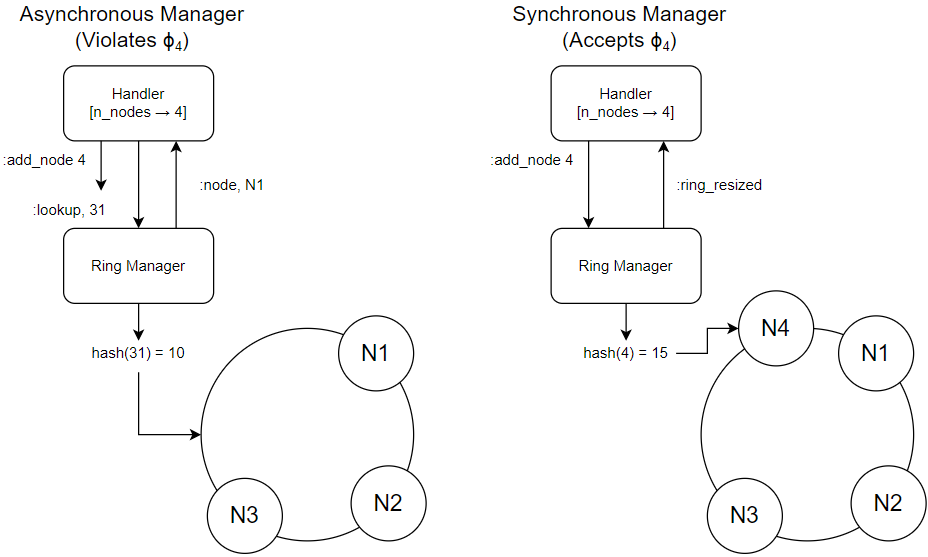
\includegraphics[width=0.8\textwidth]{images/dht.png}
    \caption{Violating and accepting consistent hash ring implementations. The violating model shows the handler sending $lookup$ requests without awaiting confirmation of ring resize. This violates the liveness property $\phi_4$, which specifically requires the manager to assign $31$ to node $4$. The accepting implementation waits for confirmation of a resize before continuing with requests. Note that $n\_nodes$ is the number of nodes the handler believes to be in the ring, not the actual number.}
    \label{fig:dht}
\end{figure}
\par
In this instance, instead of considering this an error, we may instead want to refine the system requirements. To do this, we can introduce a new liveness property to specify a weaker system, where we only care about requests being distributed to nodes.
\[
\phi_5: \square (\text{sent\_request} \rightarrow \lozenge \text{assigned\_node})
\]
Verlixir reports that $S \models \phi_5$ and $S' \models \phi_5$.
\subsection{Two-Phase Commit} \label{sec:2pc}
The two-phase commit protocol is a distributed algorithm used to update resources on multiple nodes in a single operation. It can be used to ensure replication of data is consistent across multiple nodes. For example, Spanner \cite{spanner} uses a two-phase commit between leaders of replica groups to preserve the atomicity of transactions.
\par
The protocol involves a coordinator and multiple participants. The coordinator is responsible for communicating with the participants to complete the two phases of the protocol. The first phase is the prepare phase, where the coordinator asks participants to prepare for a transaction. The second phase is the commit phase, where the coordinator asks participants to commit the transaction. In our design, the coordinator will also be responsible for terminating the participants after the transaction has been completed. When a participant is asked to prepare for a transaction, it will check the conditions it requires to commit a transaction and then reply with a $prepared$ or $abort$ message. The condition is typically application-specific, for example it could be ensuring the participant has access to a lock required for a write operation. If a single participant aborts the transaction, the coordinator will ask all participants to abort. If all participants are prepared, the coordinator will ask the participants to commit.
\par
We informally specify the system with a safety and liveness property. The safety property is that all participants must agree on the same outcome of the transaction. The liveness property is that eventually, an outcome is agreed on. We can now formalise these by constructing predicates and LTL formulae.
\[
\begin{array}{l}
\text{predicate p: commit\_count == participant\_count} \\
\text{predicate q: abort\_count == participant\_count} \\
\end{array}
\]
The $commit\_count$ is the number of participants that have committed the transaction and similarly, the $abort\_count$ is the number of participants that have aborted the transaction. The $participant\_count$ is a property specified by the system. We will reason about the protocol using a system with three participants. We can now introduce the LTL formulae to specify the system.
\begin{multicols}{2}
    \[
    \begin{aligned}
    &\textbf{SR1}: \square \left( p \rightarrow \neg \lozenge q \right) \\
    &\textbf{SR2}: \square \left( q \rightarrow \neg \lozenge p \right) \\
    &\textbf{LR1}: \lozenge \square p \lor \lozenge \square q \\
    \end{aligned}
    \]
    \vline
    \[
    \begin{aligned}
    &\text{Mutual exclusion} \\
    &\text{Mutual exclusion} \\
    &\text{Eventual agreement on commit or abort} \\
    \end{aligned}
    \]
\end{multicols}
Verlixir verifies the model is correct under these properties. We can now introduce a bug into the system. As we have mainly looked at safety properties so far, we will introduce a bug that may trigger a violation of LR1. To do this, we randomly make a participator `faulty'. Faulty participators will always abort the transaction, regardless of the coordinator's request and even if they agree to commit. We can now run the Verlixir on the updated model to see if the system violates the specification. Verlixir reports that the system violates LR1, and provides a counterexample of an execution that violates the specification. We can again use a diagram to represent the violating execution, as shown in figure \ref{fig:2pc}.
\par
\begin{figure}[h]
    \centering
    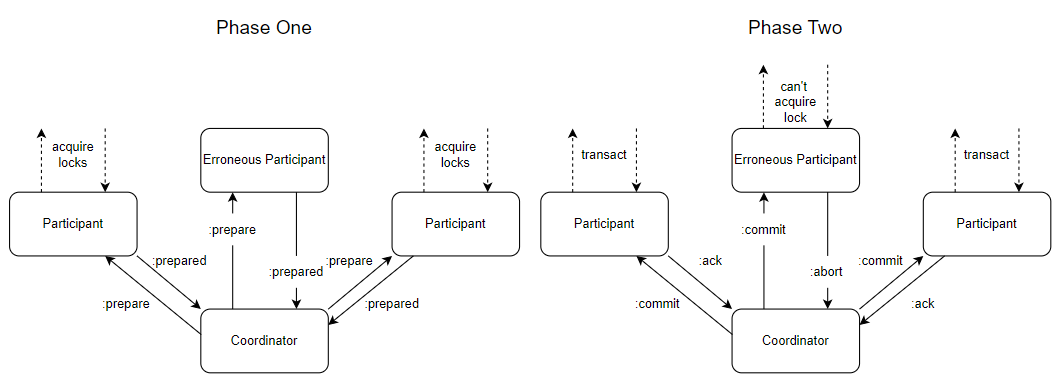
\includegraphics[width=1\textwidth]{images/2pc.png}
    \caption{Implementation of two phase commit that violates specification (LR1).}
    \label{fig:2pc}
\end{figure}
\par
We can see from figure \ref{fig:2pc}, that in the counterexample reported by Verlixir, the erroneous participant may reply to the coordinator with a $prepared$ message, before acquiring the relevant locks. This means the coordinator has the relevant information to ask participants to commit. The erroneous participant will attempt to commit, determine it does not have the required locks to do so and then abort. Verlixir reports this violates the liveness property LR1, as the system never reaches a state where all participants either commit or abort.
\par
For this counterexample, the message log produced by Verlixir makes the violation relatively obvious.
\begin{lstlisting}[xleftmargin=.01\linewidth, xrightmargin=0.01\linewidth, caption={Message log produced by counterexample violating LR1.}, label={lst:2pc_violation}]
send [1, PREPARE, ...]
send [3, PREPARE, ...]
send [5, PREPARE, ...]
...
send [7, PREPARED, ...]
...
send [7, PREPARED, ...]
...
send [7, PREPARED, ...]
...
send [1, COMMIT, ...]
send [3, COMMIT, ...]
send [5, COMMIT, ...]
...
send [7, TRANSACTION_COMMIT, ...]
...
send [7, TRANSACTION_COMMIT, ...]
...
send [7, TRANSACTION_ABORT, ...]
...
\end{lstlisting}
Listing \ref{lst:2pc_violation} shows a reduced version of the message log produced. We can see the first broadcast of $prepare$ messages is sent to all participants\footnote{The numbers 1, 3 and 5 are the process identifiers assigned to the participants by Verlixir. Although this reveals some of the internals Verlixir uses to model programs, being aware of what these are can help understanding errors. They do not have any significance in the actual program.} and subsequently the participants replying with $prepared$ messages. The coordinator then broadcasts a $commit$ message, which is received by all participants. However, in the response to $commit$ we notice that one participant sends an unexpected $transaction\_abort$ message. This explains the violation of LR1, as well as gives an indication as to where in the execution it was violated.
\subsection{Dining Philosophers} \label{sec:dp}
The dining philosophers problem is a classic concurrency problem used to illustrate the challenges of concurrent programming. The problem involves a group of philosophers sitting at a table in a circle. Between each philosopher is a fork. A philosopher can either be thinking or eating. To eat, a philosopher must first pick up both the fork on their left and right side.
\par
There are many flavours of this algorithm with increasing complexity to handle the concurrency primitives. To evaluate the expressiveness of Verlixir, we will specify the system with a naive approach:
\begin{itemize}
    \item A philosopher will ask to be sat at the table.
    \item A philosopher will attempt to pick up the fork to their left.
    \item A philosopher will attempt to pick up the fork to their right.
    \item A philosopher will eat for some time.
    \item A philosopher will put down the left fork, right fork and then leave the table.
\end{itemize}
In particular, the process algebra for a philosopher, $Phil$ is as follows:
\[
\begin{aligned}
    & \text{Phil} = ( \text{sit} \rightarrow \text{pickupLeft} \rightarrow \text{pickupRight} \rightarrow \text{eat} \rightarrow \text{putdownLeft} \rightarrow \text{putdownRight} \rightarrow \text{leave} \rightarrow \text{SKIP}) \\
\end{aligned}
\]
The issue with this approach is that if all the philosophers pick up the fork to their left, then they will all be waiting for the fork to their right. This is a known deadlock, and we would expect Verlixir to be expressive enough to detect this. When we run Verlixir on the dining philosopher specification, it reports a violation of the safety property that a deadlock should not occur. We can read the trail produced by Verlixir, to determine our understanding of how a deadlock may arise in this naive implementation, is correct.
\par
To summarise the trail produced by Verlixir, we will demonstrate a process composition for two philosophers, $Phil_0$ and $Phil_1$ that results in a deadlock. We denote the fork on the philosopher's left as $Fork_{i}$ and on the right as $Fork_{(i+1)\%n}$ for philosopher $Phil_i$, where $n$ is the number of philosophers; similarly for a fork, the philosophers are located at $i$ and $(i-1)\%n$. We will use $L$ and $R$ interchangeably to express left and right. 
\[
\begin{aligned}
    & \text{Phil}_i = (\text{sit}_{i} \rightarrow \text{pickup}_{iL} \rightarrow \text{pickup}_{iR}\rightarrow \text{eat}_{i} \rightarrow \text{putdown}_{iL} \rightarrow \text{putdown}_{iR}\rightarrow \text{leave}_i \rightarrow \text{SKIP}) \\
    & \text{Fork}_i = (\text{pickup}_{Li} \rightarrow \text{putdown}_{Li} \rightarrow \text{Fork}_{i}) \ | \ (\text{pickup}_{Ri} \rightarrow \text{putdown}_{Ri} \rightarrow \text{Fork}_i) \\
    & \text{DiningPhilosophers}(2) = \text{Phil}_0 \ || \ \text{Phil}_1 \ || \ \text{Fork}_0 \ || \ \text{Fork}_1 \\
\end{aligned}
\]
Which when ran using Verlixir, produces the violating trace:
\[
    \text{sit}_0 \rightarrow \text{sit}_1 \rightarrow \text{pickup}_{00} \rightarrow \text{pickup}_{11} \rightarrow \text{STOP} \\
\]
We can observe that even without explicitly specifying system properties, Verlixir is capable of detecting a deadlock in systems. We can now look at a shortened version of the message log produced by Verlixir to reason the counterexample produced, aligns with our intuition.
\begin{lstlisting}[xleftmargin=.01\linewidth, xrightmargin=0.01\linewidth, caption={Message log produced by counterexample of a Dining Philosophers deadlock.}, label={lst:dp_deadlock}]
    The program likely reached a deadlock. Generating trace.
    <<<Message Events>>>
    send [2,PICKUP,4]
    send [4, OK]
    send [3,PICKUP,5]
    send [5, OK]
    send [2,PICKUP,5]
    send [3,PICKUP,4]
    <<<Deadlock>>>
\end{lstlisting}
The trace in listing \ref{lst:dp_deadlock} shows four $pickup$ messages being sent. The values in these messages do not necessarily directly correspond to anything in the Elixir program, however, we can use some intuition to workout what is going on. For any message log, the first element will be the intended receiver. Hence, the first message shows a philosopher with process identifier 4 sending a $pickup$ message to a fork with process identifier 2. Continuing this logic, we can see the interleaving results in the philosophers with identifiers 4 and 5, both attempting to pickup the fork to their left. We see the forks confirming they have been acquired, before the philosophers attempt to pickup the fork to their right. This is where the trace ends, as Verlixir reports a non-terminating state has been reached and the system has deadlocked.
\par
We can see that if we map the process identifiers for philosophers and forks to the numbering system we used in the process algebra, the trace aligns with our operational semantics for the system. This gives us confidence that Verlixir is correctly identifying deadlocks in the system.

\subsection{Raft Consensus} \label{sec:raft}
The final algorithm we will use in the evaluation of Verlixir's expressiveness is Raft \cite{raft}. The Raft consensus algorithm was introduced to be a simpler consensus algorithm than Paxos. It is a consensus algorithm for managing a replicated log. The result produced is similar to multi-Paxos and is as efficient as Paxos. Unlike Paxos, Raft explicitly coordinates through a leader.
\par
We split the design of Raft into two components: leader election and log replication. We will primarily be focusing on leader election in this evaluation. The Raft design involves four process types: clients, followers, candidates and leaders. Clients communicate directly with leaders to propose log entries for replication. Leaders will commit these log messages and forward them onto followers. There can be multiple leaders at any moment, however, the Raft algorithm is divided into `terms'. If multiple leaders forward log entries to a follower, it will only respect the leader elected for the highest term. If a follower does not receive a message from a leader within a certain time frame, it will mark itself as a candidate and initiate a new leader election.
\par
Leader election involves selecting a new term number and asking all followers to vote for the candidate. If a candidate receives a majority of votes, it marks itself as the leader for the term. The consensus algorithm is designed such that only one leader can be elected per term, in the case of a split vote then no leader is elected.
\par
\subsubsection{Instrumenting Raft}
We first use Verlixir to determine we can reach consensus on a round of leader election. To do this, we configure our implementation by introducing a coordinator to initiate the first round of leader election. The coordinator does the following:
\begin{itemize}
    \item Set $n\_nodes$ = 3
    \item Set $n\_rounds$ = 1
    \item Spawn 3 followers
    \item Bind a unique new term number to each follower
    \item Broadcast a $start\_election$ message to all followers
    \item Await an $elected$ message from a leader
\end{itemize} 
We instrument the program in such a way that we enforce an election to take place, and with our intuition of the Raft algorithm, as all the followers have unique term numbers, we expect one of them to be elected as the leader (the follower with the highest unique term number). With the system instrumented in such a way, the only liveness requirement we are interested in is the eventual termination of the program (considering the program will only terminate when the coordinator receives an elected message). When we run Verlixir on the instrumented program, we observe every execution is a terminating one. This gives us confidence the Raft specification is able to reach consensus on a leader.
\par
\subsubsection{Introducing Timeouts}
Next, we slowly expand our system requirements and incrementally test correctness as we go. Instead of instrumenting the system with a coordinator to begin an election, a true Raft system will automatically begin rounds of leader election. Raft does this using timeouts. Every participant in the system is able to initiate an election if they fail to receive a message from the leader within a specified time frame. We can now introduce this behaviour into our system. The coordinator no longer broadcasts a $start\_election$ message; instead, the followers will rely on the timeout to initiate elections. We again run Verlixir on the updated model, and observe that the system is still able to reach consensus on a leader (as determined by termination).
\par
\subsubsection{Safety Requirements}
To complete our consensus specification, we are interested in the following safety requirement:
\begin{itemize}
    \item \textbf{SR}: Only a single leader is elected per term.
\end{itemize}
Although up to this point we have shown the liveness property, that the system eventually terminates with a leader holds, this is not actually a guaranteed requirement of the system. Due to split-votes, we cannot always guarantee election. What we can guarantee is that if a leader is elected, it is the only leader for that term.
\par
We introduce the SR into our system by increasing $n\_rounds$ so that we can observe multiple participants being elected as leaders. We can then introduce the SR formally with LTL:
\[
\text{SR} = \square ( \text{elected\_term} \neq \text{previously\_elected\_term} )
\]
LTLixir does not explicitly support the ($\neq$) operator, so we can rewrite the SR in LTLixir as:
\begin{lstlisting}[language=Elixir, xleftmargin=.3\linewidth]
@ltl """
!<>[](elected_term == previously_elected_term)
"""
\end{lstlisting}
This is a more implementation-specific approach. We can run the system with $n\_rounds$ as 2, then the variables will be set to the values of the two rounds. The LTL will hence ensure that we never always have an execution where the elected terms were equivalent.
\par
We can finally verify the system with this property and determine the system is correct with respect to our specification.
\section{Verlixir vs. Existing Work} \label{sec:vs}
We will now compare Verlixir to existing state-of-the-art work in verification-aware languages and modern programming language verification tools. We believe Verlixir is the first tool to support a pure message-passing model of computation, and hence much of the design has introduced novel techniques to support this. We will first discuss some of these techniques that differentiate Verlixir from existing work. We will then provide a direct comparison between Verlixir and existing tools, before discussing the future of Verlixir.
\subsection{Difference in Approach}
Verlixir is the first verification-aware language to support a pure message based model. This is a significantly different approach to existing tools, which have either ignored concurrency, used shared-memory models or communication over channels. 
\par
To support a shared-nothing model, we ensure all heap memory is kept local to processes and all data sharing is achieved explicitly through communication. We applied heuristics to bound the communication possible between processes, by modelling infinite mailboxes as finite Promela channels. A challenge with a shared-nothing model is supporting passing data structures. To support this, we introduced a technique to pass data structures between processes by storing data structures in a global memory and providing processes with pointers to access and send structures through messages. 
\par
Any Elixir function can be used to spawn a new process. Elixir functions are also often highly recursive. To handle both the spawning and recursion of a function, we introduced a method to determine the nature of a functions usage at runtime and instrument the behaviour depending on the function's usage. For example, a function being spawned as a new process needs to determine a unique process identifier, whereas a function being called naturally needs access to the parents process identifier and also needs to communicate with the parent through a rendezvous channel to ensure the parent waits for the child to complete.
\par
Elixir also uses a receive-anything pattern, where due to the language's dynamic typing and matching, determining how a message should be processed can involve peeking into the message to examine its contents. To enable verification of this, we introduced a method to process messages in a non-blocking manner, where messages can be received and parsed in a first-in-first-fireable-out (FIFFO) order.
\par
To give a higher level overview of where Verlixir differentiates itself from existing tools, we provide a table of comparison in table \ref{table:vs}.

\begin{table}[ht]
    \centering
    \begin{tabular}{|>{\raggedright\arraybackslash}p{4cm}|c|c|c|c|c|}
        \hline
        \textbf{} & \textbf{Verlixir} & \textbf{Java PathFinder} & \textbf{Gomela} & \textbf{Dafny} & \textbf{Lean} \\
        \hline
        Concurrency & Actor-based & Shared-memory & Channel-based & \xmark & \xmark \\
        \hline
        Propositional logic & \cmark & \text{Limited} & \xmark & \cmark & \cmark \\
        \hline
        Predicate logic & \xmark & \xmark & \xmark & \cmark & \cmark \\
        \hline
        Temporal logic & \cmark & \xmark & \xmark & \xmark & \xmark \\
        \hline
        Model checking & \text{SPIN} & \text{SPIN \footnote{The original Java PathFinder (JPF) design modelled programs in SPIN \cite{jpf}.}} & \text{SPIN} & \xmark & \xmark \\
        \hline
        Theorem proving & \xmark & \xmark & \xmark & \text{Z3} & \text{Built in} \\
        \hline
        LTL & \cmark & \xmark & \xmark & \xmark & \xmark \\
        \hline
        Safety & \cmark & \text{Deadlock} & \text{Deadlock} & \xmark & \xmark \\
        \hline
        Liveness & \cmark & \xmark & \xmark & \xmark & \xmark \\
        \hline
    \end{tabular}
    \caption{Comparison of Verlixir to existing tools.}
    \label{table:vs}
\end{table}
\subsection{Translation Results}
A large component of Verlixir is the translation of Elixir to Promela. As Verlixir is the first of its kind, we have no benchmark to evaluate the translation progress. However, we can provide insights into the translation process, results, and future work.
\par
Verlixir was primarily designed to suit any backend. In particular, concurrent model checkers such as SPIN, PAT or PRISM. Given SPIN is the targetted model checker, we introduced some SPIN specific optimisations to the design in order to reduce the state space and time complexity of model checking. For example, consider how we optimised the modelling over the Elixir mailbox over multiple iterations:
\begin{itemize}
    \item \textbf{Singular Mailbox}: the original mailbox was designed such that every process has its own mailbox (alike to Elixir). Receiving messages involved the same approach Elixir uses. Messages were stored in a FIFO queue. To receive a message, we scan the queue pushing to a stack, until we find a message that matches the pattern. We can then take the message from the queue, and re-apply the stack. 
    \item \textbf{Multiple Mailboxes}: we optimised this approach to reduce scanning by splitting the mailbox up such that each possible message type in the system has its own, per-process mailbox. This reduces the time required to search the state-space as channel orderings are more deterministic. 
    \item \textbf{Random read, sorted insert}: we further improve by moving from sequential select $?$ Promela's random select $??$ operator to match messages in the mailbox. We do this to reduce the number of process interleavings that need to be explored in the state-space. Finally, now we are using random select, we can also use sorted insert $!!$. Because we are reading randomly, the order of messages in the mailbox is not important, so by sorting the mailboxes we reduce the state-space. 
\end{itemize}
\subsubsection{Forward Optimisations}
There is lots of scope to further optimise the translation process. The existing framework has been designed such that this is easy to achieve. For example, we currently translate all Elixir functions to Promela functions. This incurs an overhead that may not be strictly necessary. By statically analysing the behaviour of a recursive function, we could apply heuristics to unroll the recursion and inline the function using an imperative style loop.
\par
As alluded to earlier, there is room to replace the SPIN backend with another model checker. Although we identified SPIN sufficient for our purposes, as explored in section \ref{sec:model_checking}, other model checkers support features that SPIN does not. For example, probabilistic model checkers can more accurately model systems that involve randomness, such as gossip protocols. We aim for the design of the IR to be flexible enough to support swapping out backends. 
\section{Summary}
This chapter has highlighted the expressiveness of Verlixir by modelling and verifying distributed algorithms that are frequently used in both industry and academia. We have shown the toolchain is capable of supporting these specifications, verifying properties over them and providing clear feedback when properties are violated. We have also compared Verlixir to existing tools, highlighting the differences in capabilities provided for various verification-aware languages. Finally, we have evaluated the translation process from Elixir to Promela, providing insights into the optimisations that have been made and the potential for future work.